\documentclass[11pt, oneside]{article}   	
\usepackage{geometry}                		
\geometry{letterpaper}                   		 
%\geometry{landscape}                		
%\usepackage[parfill]{parskip}    		
\usepackage{graphicx}				
										
\usepackage{amssymb}
\setlength{\parindent}{0pt}
\title{Summary Paper of A Novel Approach to Short-Term Stock Price Movement Prediction using Transfer Learning}
\author{Jody Shu}
%\date{}							% Activate to display a given date or no date

\begin{document}
\maketitle
%\section{}
%\subsection{}
\begin{Large}
The paper describes a base model using long short-term memory (LSTM) cells is pre-trained based on a large amount of data, which are obtained from 50 different stocks, to optimize initial training parameters, and then use the results from the trained model as initial values to further train a smaller samples from the target stock (COI).  Furthermore,  the LSTM model can lessen the problem of vanishing (and exploding) gradients.The inputs for the pre-processed base model is constructed based on the relationship between stocks. These input features are based on the following:\\

\begin{itemize}
\item One-day returns of the COI stock. 
\item Combination of one-day returns of COI stock and the index (e.g.,
Korea Composite Stock Price Index 200 (KOSPI 200) and Standard $\&$ Poor's 500 (S $\&$ P 500). 
\item Combination of one-day returns of the COI stock, the index, and stocks related to the COI stock (i.e., the highest cosine similarity (CS) to the COI stock, similar field (SF) to the COI, and the highest
market capitalization (HMC)).
\end{itemize}

The reasons for choosing these above-mentioned relationship, the authors stated that \\
"CS selects stocks that have a direction in closing price movement that is most similar to the COI stock; SF finds stocks that have similar industrial products to the COI, even though there may be no direct closing price movement correlation between them; and HMC aims at choosing the largest companies in each stock market $\ldots$ the performance of the SF selection method substantially dominates other considered methods in terms of average prediction accuracy."\\


Moreover, they used data from top-five companies in the Korean market and the United States (US) market from 2012 to 2018 in terms of the highest market capitalization.  The result of the experiments showed promise for the effectiveness of transfer learning by efficiently using stock correlation information to further improve model performance.  In addition, the authors also compared with other benchmark methods to demonstrate the prediction accuracy of the model using stock time series data.  These three baseline models which the authors compared against their model are as follows:
\begin{itemize}

\item Artificial neural networks (ANNs)
\item Support vector machines (SVMs)
\item Random forests (RFs)
\end{itemize}
\section{Long Short Term Memory Description}
Figure 1,  $x_t, h_t, and\ c_t$ are defined as the input, the hidden state, and the cell state at time t respectively.  An LSTM cell has three gates: $f_t, i_t, and  \ o_t$, which are called the forget gate, the input gate, and the output gate, respectively. $\otimes$ is point-wise multiplication. Sigmoid and tanh activation functions are marked as
$\textit{sigmoid}$ and\ $\textit{tanh}$, respectively.  tanh(z) =$ \frac{2}{1+e^{-2z}}-1, \sigma(z)=(1+e^{-z})^{-1}$
The sigmoid function helps form the output value in the range of [0, 1]. If the output is close to 0, most information is lost.  If the output value is close to 1, it means that more information is allowed.   Please see the graph below.

\begin{figure}[h!]
  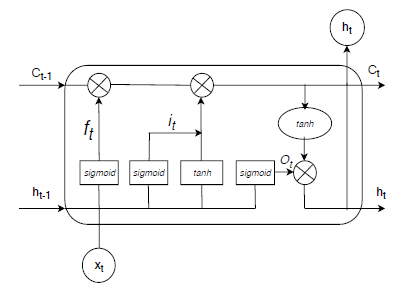
\includegraphics[width=150mm,scale=0.7]{fig1.png}
\end{figure}

The following shows the formulas for calculating forget gate\ $ (f_t), the\ input \ gate \ (i_t), \\
the \ output\ gate\ (o_t), the \ cell \ state \ (c_t) \ and \ the \ hidden\ state\ (h_t) $\\

$f_t=\sigma(W_f\ast x_t+U_f\ast h_{t-1}+b_f)$\\
$t_t=\sigma(W_i\ast x_t+U_i\ast h_{t-1}+b_i)$\\
$o_t=\sigma(W_o\ast x_t+U_o\ast h_{t-1}+b_o)$\\
$c_t=f_t\ast c_{t-1}+i_t \ast tanh(W_c \ast x_t+U_c \ast h_{t-1}+b_c)$\\
$h_t=o_t\ast tanh(c_t)$

where $W_f,W_i,W_o,W_c,U_f,U_i,U_o$ and $U_c$ are weight matrices, and $b_f,b_i,b_o$ and $b_c$ are bias vectors.\\
%
Transfer learning is a type of machine learning techniques to extract the feature from a large data more efficiently, and in this paper, the authors used inductive transfer learning since the labeled data in both the source data and the target data are available.  In addition, there are four different transfer learning setting (i.e., instance-transfer, feature-representation-transfer, parameter-transfer, and relational-knowledge-transfer), and among them, parameter-transfer was chosen for this research.\\

\section{Dataset, Preprocessing and conclusion}

According to the paper, $r^{\mathrm{s}}_{t,p}$ is Return of stock s on day t over the previous p days (i.e., the difference in closing price between day t and day (t - p) as follows:\\

\hspace{30pt}$r^{\mathrm{s}}_{t,p}=\frac{P^{\mathrm{s}}_{t} - P^{\mathrm{s}}_{t-p}}{ P^{\mathrm{s}}_{t-p}}$\\
%
\\Feature vector: $R^{\mathrm{s}}_{t}=\{r^{\mathrm{s}}_{t-19,1}, r^{\mathrm{s}}_{t-18,1},\ldots, r^{\mathrm{s}}_{t,1}\}$

$y^{\mathrm{s}}_{t} $ \ is an indicator of the output for the estimation model.  For example,
$y^{\mathrm{s}}_{t} $= 1 indicates that an increase in the closing price on day t + 1, compared to the previous day, and $y^{\mathrm{s}}_{t}$= 0 means a decrease in the closing price.\\
%
As the paper stated to train the base model are the following: \\

The first step is preparing a large source of data obtained from 50 available stocks. 
The second step is the training process. \\ Without going into the details, below is the figure to demonstrate the structure of the data.

\begin{figure}[h!]
  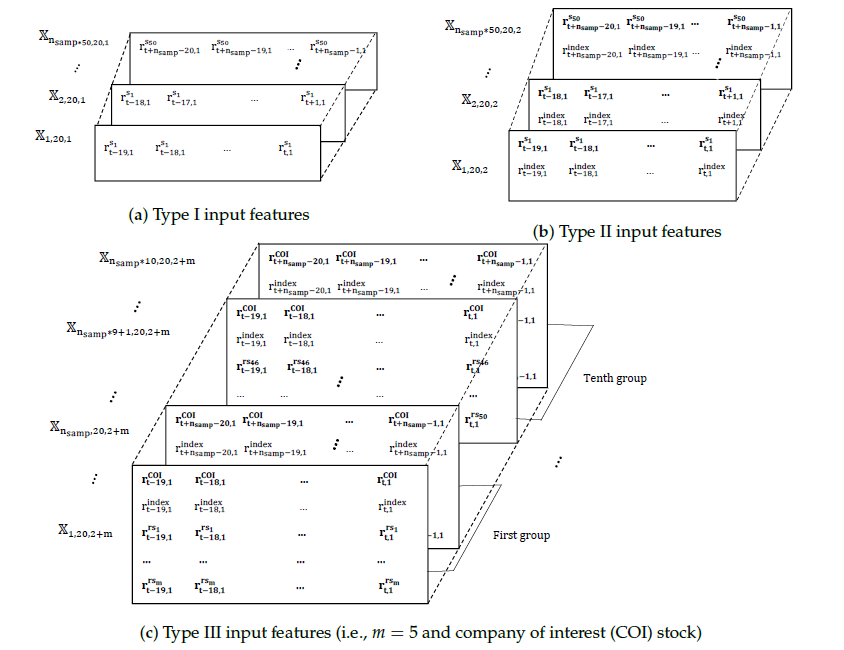
\includegraphics[width=180mm,scale=0.8]{fig2.png}
\end{figure}

Simply put, the authors stated the training process as follows:

For training the base model, a variety of network architectures which have a different number of
layers, hidden units, and activation functions were examined. Then, from among the considered
configurations, the most appropriate network architecture was selected based on the highest
performance over the validation set. The topology of our LSTM model is as follows:
\begin{itemize}
\item The input layer has units that equal the number of features and 20 time steps.
\item There are two LSTM layers, which are followed by two fully connected layers. 
Each layer has 16 units and dropout regularization is applied to the outputs of each
hidden layer in order to mitigate the overfitting problem. Keep probability values are set to 0.5.
\item The output layer has one sigmoid activation unit.
\end{itemize}

In training the prediction model, six dimensional tensors, $\mathbb{SI}_1, \mathbb{SI}_2,\\
 \mathbb{SI}_{3a}, \mathbb{SI}_{3b}, \mathbb{SI}_{3c}, and\ \mathbb{SI}_{3d}$
with dimensions of n samp $\times 20 \times k$ are constructed as the training data for six types of input vectors which is fed to each model as base model.  Please see below.

\begin{figure}[h!]
  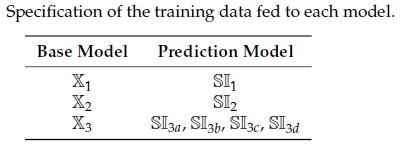
\includegraphics[width=150mm,scale=0.8]{fig3.png}
\end{figure}
The subgroup m, randomly divide up by 3,5, or 7 in each group among the 50 stocks. Therefore, m=$\{3,5,7\}.$. And this has also affected the effectiveness of the prediction.\\

The final experiment demonstrated that the model is successful to predict the movement of the stock price.  Please see the comparison as below.

\begin{figure}[h!]
  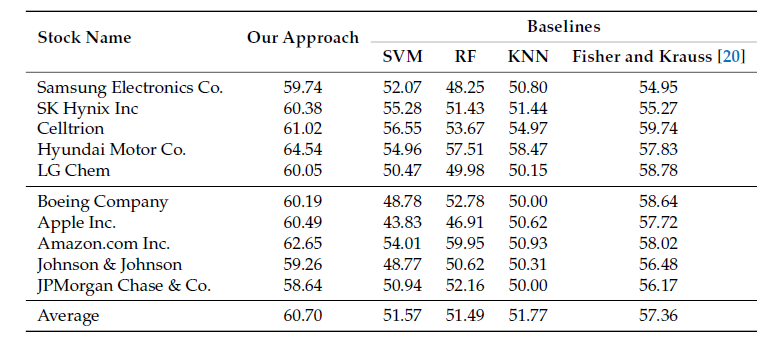
\includegraphics[width=160mm,scale=0.5]{fig4.png}
\end{figure}

\end{Large}
\end{document}  